\documentclass[12pt, a4paper]{article}

\title{Weave\\Business Plan}
\date{05/05/2017}
\author{Z0972973}

\bibliographystyle{apacite}

\usepackage{fancyhdr}%Headers
\usepackage{setspace}%1.5 Spacing
\usepackage[toc, page]{appendix}%Appendices
\usepackage{titling}%Used to fix abstract to go on same page
\usepackage{geometry}%center cover page
\usepackage[switch]{lineno} %line numbering
\usepackage[T1]{fontenc} %make vertical pipe | work
\usepackage[british]{babel}%hyphenation
\usepackage{url}
\usepackage{varioref}%Automatic page references
\usepackage[colorlinks, allcolors=blue]{hyperref}%Automatic reference links
\usepackage[capitalise]{cleveref}%Automatic reference typing
\usepackage[sectionbib, tocbib, numberedbib, bibnewpage]{apacite}%Citations
\usepackage{titlesec}%Title spacing
\usepackage{graphicx}%PDF insert
\usepackage[section]{placeins}%Place figures in section they're defined in
\usepackage{multicol}%multi column bib
%\usepackage{pdflscape}
\usepackage{colortbl}
\usepackage{booktabs}
\usepackage{rotating}
\usepackage{tablefootnote}
\usepackage{multirow}
\usepackage[bottom]{footmisc}
\usepackage{threeparttable}
\usepackage{tikz}
\usepackage{pgfplots} % for graphing
\usepackage{pdfpages}
\usepackage{subfig}

\pgfplotsset{compat=1.13}

\let\cite\shortcite

\pagestyle{fancy} %set header
\makeatletter
\let\runauthor\@author
\let\runtitle\@title
\makeatother
\rhead{\runauthor}
\lhead{\runtitle}

\newcounter{TableFootnoteStart}
\newenvironment{autotablenotes}{\begin{tablenotes}\setcounter{footnote}{\value{TableFootnoteStart}}}{\end{tablenotes}}
\newenvironment{autothreeparttable}{\begin{threeparttable}\setcounter{TableFootnoteStart}{\thefootnote}}{\end{threeparttable}}
\newcommand{\autoitem}{\stepcounter{footnote}\item [\thefootnote]}
\newcommand{\autonote}{\stepcounter{footnote}\tnote{\thefootnote}~~}

\setlength{\headheight}{28pt} %Set header to be big enough

\titlespacing{\section}{0pt}{0pt plus 2pt minus 2pt}{0pt plus 2pt minus 2pt}
\titlespacing{\subsection}{0pt}{0pt plus 2pt minus 2pt}{0pt plus 2pt minus 2pt}

\definecolor{lgrey}{RGB}{220, 220, 220} % used for tables alternating rows
\definecolor{green}{RGB}{20, 230, 20} % For gap analysis

\newenvironment{main}
{\begin{spacing}{1.2}\setlength{\parskip}{0.5\baselineskip}}
{\end{spacing}\setlength{\parskip}{0pt}}

\begin{document}

\begin{titlingpage}
\maketitle

\begin{center}
Word Count: 3139
\end{center}

\vfill
\begin{abstract}
This business plan was prepared with a view to procure funding of \pounds 50,000 from a business angel with experience in bring apps to market and building a user base.
\end{abstract}
\end{titlingpage}

\tableofcontents
\listoftables
\listoffigures
\newpage

\begin{main}
\section{Executive Summary}
Weave is a revolutionary new dating app that combines a machine learning algorithm with locative media to introduce you to people as you go about your day. Weave takes a current trend of personality-based dating to the next level, allowing users to build real connections with people in real life.

Weave was founded in September 2016 as a limited company. Weave is owned 90\% by the founder, and the remaining 10\% is owned by the two other developers. Three developers currently work on the app and a prototype has been completed. A limited test launch is expected in August 2017 in three UK university campuses and a full launch is scheduled for October 2017.

The aim of Weave is to bring the app to market successfully, and to grow the user base through a large advertising campaign, before selling the company in its entirety in early 2018.

There are no plans to implement any revenue producing features. Advertising appears very viable as the extensive information collected about users in order to match them could also be used to target advertisements. However, Weave believes that effort would be better spent growing the user base, and not risking turning users away with ads.

The greatest risks to Weave's success were identified as the risk of user privacy concerns making users wary of installing the app and giving away their personal data, and the risk of a leak of user data leading to large fines.

\section{Company Profile}
\subsection{Business Overview}
Weave is a mobile dating app that matches based on personality with minimal input from the user. Weave was established in September 2016 and an initial prototype of the app is complete.

Dating apps have long been focussed on looks and first impressions. Weave capitalises on the emerging counter-culture of personality-based dating services. There is no such thing as scrolling through profiles, and first impressions are done in person. Weave's key value proposition for the user is a focus on in-person meeting.

Weave is designed from the ground up to minimise ongoing costs of business. The app is built around a peer-to-peer network, meaning every user acts as a server, minimising the number of centralised servers hosted by the business. Advertising is a very lucrative opportunity with Weave, as the match algorithm can also use the collected user data to ``match'' users to adverts.

\subsection{How Weave Works}
Weave's core is a machine-learning algorithm that connects two users based on how they answer a set of questions, and how they express themselves on social media. When the app is first installed, the user fills in questions and optionally gives Weave read-only access to their public social media accounts. Then, the user puts their phone away and goes about their day.

As the user walks around, Weave constantly looks for other users using Bluetooth\footnote{Bluetooth LE is the low-energy version of Bluetooth, meaning the app will consume minimal battery on the user's phone \cite{BluetoothLE}}. When another user is found, the phones automatically determine whether the users are a match. If they are, both phones vibrate and ask whether their user has time to talk to a match. If both users say yes, the phones guide the users together. This is the first time they have seen each other, and they still know nothing about each other. The users are encouraged to chat, and afterwards to rate the match. This rating is used to improve the machine learning algorithm automatically.

\subsection{Company History}
Weave was created in September 2016, after promising preliminary market research and a successful start to prototyping the app. Steven, the founder, quit his job and re-mortgaged his house to begin working on Weave full time. In February 2017, a programmer specialising in machine learning was hired to develop the underlying match algorithm. In late March 2017, an additional front-end developer was hired to work on the design and development of the user interface and user experience. Today, a working prototype of the app has been developed, demonstrating its functionality and design.

\section{Business Analysis}
\subsection{Risk Analysis}
A Risk Analysis was performed (see \cref{app:Risk}) to identify major areas of risk in the business. The main risk identified was the risk of a security flaw in the app leading to a leak of user data. A leak of ``personal data'' can lead to a multi-million Euro fine under EU regulation \cite{EuDataProtection}.

This risk will be mitigated by following best practices in storing and transmitting private data, and by only storing the data on the user's device, which also reduces storage costs. A firm will be hired before the app launch to check for vulnerabilities in the app that could lead to a leak of user data.

\subsection{Business Model Canvas}
The Business Model Canvas completed in \cref{app:BMC} highlighted a number of key areas of focus, including the quality of the matches, keeping the app updated so that it works on as many user devices as possible, and keeping staff happy so that they don't quit, leading to a huge time loss in training new staff. A minimum viable product (MVP) was also established as an app which uses surveys to match users automatically with other users that are nearby.

\subsection{SWOT Analysis}
A SWOT analysis was performed in \cref{app:SWOT}. Weave's strengths extended to its low cost and ability to create great matches automatically. The main weakness identified was that users are not actively using the app for very long, and will stop using it once a match is made. Users' privacy concerns were identified as the main threat to Weave's success.

\section{Market Research}
Dating apps have exploded in popularity \cite{Mintel}, especially looks-based, Tinder-like apps (see \cref{app:Competitors}), based entirely on first impressions. Since the launch of Tinder, a counter-culture has emerged, with apps being released that focus on building real connections with people (see \cref{app:MarketGap}).

Indeed, physical looks were ranked as only the fourth most important trait in a potential mate, after kindness, exciting personality, and intelligence. Approximately 14\% of males and 3\% of females valued physical looks the most \cite{LooksVsPersonality}.

\subsection{Porter's Five Forces}
The Porter's Five Forces analysis performed in \cref{app:PFF} revealed intense competition in the industry. The incredibly high fixed costs and almost zero variable costs lead to a market where every user is fought over. In addition, it was highlighted how much power Google and Apple have, with their ability to unilaterally adjust their revenue cut, or simply remove the app from their stores. There is also little stopping users from switching to another dating app. It is clear that in order to succeed, Weave must be the best, producing the best matches, and suiting the needs of its users.

\subsection{PESTLE Analysis}
A PESTLE analysis was performed in \cref{app:PESTLE}. The analysis was dominated by a prevailing theme of explosive expansion in the industry, ubiquitous use of smartphones, and a social and physical environment ripe for Weave to capitalise on. The macro-environment is perfect for Weave to be introduced into.

\subsection{Market Gap Analysis}
A market gap analysis was performed in \cref{app:MarketGap}. It is clearly evident the intense competition that has appeared in the personality-based dating app sector. However, it is also clear how Weave attempts to push farther than any other app, with its complete focus on personality.

\subsection{Company Goals and Objectives}
A number of milestones have been established to provide a time-line for the successful operation and launch of the app.

\begin{itemize}
	\item \textbf{By June}, have the app developed to the point that it could be released. This will be achieved by continuing work within the team. Stop working remotely and rent an office to allow for better communication within the growing team.
	\item \textbf{By July}, fully prepare the app for launch. Focus groups must be conducted to determine how the design should be improved.
	\item \textbf{By July}, employ a marketing professional to work on the marketing surrounding the launch of the app.
	\item \textbf{By August}, launch the app in a small test environment, focussing marketing efforts on three university campuses.
	\item \textbf{By October}, redesign and improve the app based on feedback in the test environment. Expand the programming team and port the app to iOS such that it can be used on both major mobile operating systems. Officially launch the app with significant marketing efforts in universities around the country.
	\item \textbf{In Early 2018}, sell the business in its entirety to a 3rd party.
\end{itemize}

\subsection{Vision and Mission}
Weave aims to radically change what is expected from a dating app. Users should be so confident in the app's algorithm that they trust it over their own instincts. If Weave manages to bring together people that would never have given each other a second look, it has done its job.

\subsection{Legal Structure}
The business is structured as a limited company, to allow for greater protection in case of insolvency \cite{CorporateInsolvency}. This also allows the sale of shares, necessary for you to invest in the business and for offering equity to potential employees \cite{SellingShares}. As the exit plan for the business involves the sale to a third party, the shareholder's agreement contains a "drag-along" clause to allow for sale of 100\% of the business \cite{DragAlongClause}.

Staff currently own 10\% of the business. To mitigate the risk of staff leaving and taking their shares, their work contracts contain a clause which makes them give up their shares should they leave before January 2018.

\subsection{Location}
Currently business is conducted entirely remotely to reduce operating costs with occasional meetings in cafés and public areas. Weave aims to move to a modest office in June 2017 to accommodate new staff and bring the employees together physically before the test launch. Programming is easily done remotely but other activities such as marketing benefit from the close proximity of staff.

Weave's users will be spread all around the world. The app works best when many users are grouped closely together, so it will inevitably be more popular in cities and population centres. The initial test launch in August will concentrate on three UK university campuses to maximise the potential user concentration.

\subsection{Intellectual Property}
All of the code used in the app is automatically protected by copyright upon its completion \cite{CodeCopyright}. This provides legal protection from other apps copying the code or algorithms used in the app. The visual design of the app will also be automatically copyrighted separately, meaning that an exact visual clone of the app would be unlawful \cite{ArtCopyright}.

In the case that work is copied illegally, the costs of legal action may be prohibitive. To reduce the costs of legal action, the artwork and code will be registered with the UKCS, the UK Copyright Service. This means that in the case of legal action, the government has a verifiable copy of the work at the time it was registered \cite{RegisteredCopyright}. The cost of registering a work is \pounds 72.50 \cite{CopyrightCost}, and updating the work costs \pounds 19.50 \cite{CopyrightUpdateCost}. These costs are economical when considering the future inconvenience that is prevented.

Copyright does not prevent an app with similar functionality from being implemented, it simply provides legal recourse in case the exact implementation has been copied. A competing company could use "Clean Room Design", in which the app is reverse-engineered and reimplemented from scratch, to recreate the app without violating copyright \cite{CleanRoomDesign}. However, they may still have violated the design rights, which cover the general look-and-feel of the app \cite{ArtCopyright}.

\section{Personnel}
\subsection{Current Personnel}
\begin{itemize}
	\item Steven Lowes, Founder, Developer. Steven founded Weave in 2016 and currently works on implementing the user discovery functionality. His full CV is available in \vref{fig:StevenCV}.
	\item Kennard Upton, Back-end Developer. Kennard joined Weave in February 2017 and is developing the match algorithm. He has extensive experience in machine learning, working at Google to develop the advert targeting algorithm for YouTube. Ken took a lower salary along with a 7\% share of the company to work for Weave. His full CV is available in \vref{fig:KennardCV}.
	\item Lindsey Bennett, Front-end Developer, Artist. Lindsey joined Weave in March 2017 and is developing the app front-end, user experience, and art style. Lindsey's most notable work is her part in the design of the front-end of BBC iPlayer. Lindsey took a lower salary along with a 3\% share of the company to work for Weave. Her full CV is available in \vref{fig:LindseyCV}.
\end{itemize}

\subsection{Future Plans}
\begin{itemize}
	\item \textbf{Developers:} Weave aims to hire two additional developers after the test launch to work on a port of the app for iOS, allowing the app to run on Apple devices.
	\item \textbf{Marketing:} Market share is of utmost importance to Weave's functionality. With this in mind, a large marketing effort is planned before release. Weave will hire three marketing professionals to design and implement this campaign. A marketing firm could be hired additionally if a larger advertising effort is needed on short notice.
	\item \textbf{Research:} Before the full launch of the app, it is important that the user experience is designed with the users in mind. A two-man research team will focus on finding improvements for the app based on user feedback and focus groups. This team will also keep track of industry trends to provide strategic information guiding the company into the future.
\end{itemize}

\subsection{External Personnel}
Some tasks are needed so rarely that it does not make economical sense to hire an employee full time for that task. Expertise is therefore outsourced when needed to fill these roles. Situations in which external personnel are brought in currently extend to Accountancy and Legal services.

\section{Branding and Marketing}
\subsection{Branding}
Weave's name was chosen for a number of reasons:
\begin{itemize}
	\item Taken literally, the app weaves its way through your life, and the interactions you have with other people.
	\item Weave promotes imagery of threads, akin to the 'thread of fate' spun by the Greek and Roman goddesses of fate. This focus on fate was meant as a tongue-in-cheek reference to the fact that Weave is there for you when fate/destiny falls short.
	\item Dating app names must be easily memorable and short. One-word names are the norm.
	\item The name is not used by any other major app.
\end{itemize}
Weave's logo is currently in development.

\subsection{Advertising}
A major source of public awareness of Weave will be word-of-mouth and chance encounters. Seeing people walking along, then pulling out their phones, turning around, and meeting someone will be so unusual that when that person eventually learns about Weave, they should remember that event, making the app immediately appear popular. In addition, the app is so unique that users will talk to their friends, demonstrating the new technology in use. The app is free to use, so the friends will likely install the app to try it too.

Of course, word-of-mouth will not be sufficient to build a user base. Weave envisions the advertising campaigns used to be a combination of formats. Examples of planned channels include articles in blogs, especially tech blogs, in addition to news-like sites such as BuzzFeed and maintaining a strong social media presence. 

\subsection{Markets Served}
It is feasible that Weave, in some future incarnation, could serve as the main mechanism through which people discover potential partners. Indeed, a large user base is essential to the effective functioning of the app. However, it is understood that such a goal is impossible in the short-term, and that a more targeted approach is initially required.

\subsubsection{Initial}
The market that will be targeted initially is university/college students. This market was selected primarily for its incredibly high density of potential users. 91\% of 18-44 year olds in the UK own a smart phone \cite{DeloitteMobileConsumer}, and will be very densely packed on the university campus, meaning that the app will find more potential matches. University students are often prime romantic partners, due to them being single more often than other groups \cite{ONSMarriage}, and having similar education levels, economic status, and of a similar age. 

\subsubsection{Future Plans}
Those aged 18-24 are most likely to use online dating, but over one fifth of adults aged 18-44 use online dating \cite{AgeRanges}. Weave's archetypal user sits in this age range, is a busy professional with little time to spend sifting through profiles, and is put off by the superficial nature of other dating apps. However, the app could have a wide reach outside of this group, and will be tailored to the people that end up actually using the app through frequent focus groups and examining user data.

\section{Finances}
The start-up funds of \pounds 51,000 were investment by from the founder, which has been sufficient until now due to Weave's lean operation. In order to expand the company and bring the app to a test market, Weave is requesting \pounds 50,000 of investment from you in exchange for a 15\% share of the company. It is expected that future investment of \pounds 300,000 will be sought before the full launch in October.

\subsection{Revenue Streams}
It is not expected that Weave will generate any revenue until after it is sold. There are various revenue streams available, such as targeted advertisements, which appear very lucrative (see \cref{app:AdRevenue}). However, Weave determined that taking the time to implement any revenue generating features would slow development and delay the app's launch, in what is a very fast-moving market \cite{Mintel}.

Weave understands that the most valuable part of the business is the user base, and there is little concern over the app's ability to turn a profit once the user base is established and the app entrenched in the industry. When 1 in 4 users only open an app once, and only 38\% use it more than 10 times \cite{AppRetention}, Weave is wary of implementing intrusive ads that could  turn users away. Weave's focus is decidedly on creating value rather than profit. Ignoring revenue streams until the app is established is a tried-and-tested route for dating apps \cite{TinderPrice, BumblePrice, GrindrPrice}.

\section{Conclusion}
Weave is unlike any other app and could change the way we think about meeting people, by matching users together with incredible accuracy and becoming the de-facto standard in the industry. The more popular Weave is, the better the underlying algorithm will be at picking the best match. There is unbounded potential for growth, and Weave has the opportunity to become the dominant force in the personality-based dating sector, which is heavily contested but with no real leader. Your investment has the capacity for huge returns in under one year, and will allow Weave to change the world.

\newpage

\begin{appendices}
	\section{Current Staff CVs}
	\label[appendix]{app:CVs}
	\subsection{Steven Lowes}
	\label[appendix]{app:StevenCV}
	Steven Lowes is the founder and general Java developer for Weave. He owns 90\% of the business. His CV is available in \vref{fig:StevenCV}.
	\begin{figure}
		\begin{center}
			\caption{Steven Lowes' CV}
			\label{fig:StevenCV}
			\includegraphics[width=0.95\columnwidth]{CVs/steven.pdf}
		\end{center}
	\end{figure}
	
	\subsection{Kennard Upton}
	\label[appendix]{app:KennardCV}
	Kennard Upton is the machine learning expert at Weave, working on the underlying algorithm for the app. He began working at Weave in February 2017, after meeting Steven online and becoming interested in the app. He owns a 7\% share of the business. His CV is available in \vref{fig:KennardCV}.
		\begin{figure}
			\begin{center}
				\caption{Kennard Upton's CV}
				\label{fig:KennardCV}
				\includegraphics[width=\columnwidth]{CVs/kennard.pdf}
			\end{center}
		\end{figure}
	
	\subsection{Lindsey Bennett}
	\label[appendix]{app:LindseyCV}
	Lindsey Bennett is the front end designer and artist for Weave. She began work in March 2017, and owns a 3\% share of the business. Her CV is available in \vref{fig:LindseyCV}.
		\begin{figure}
			\begin{center}
				\caption{Lindsey Bennett's CV}
				\label{fig:LindseyCV}
				\includegraphics[width=\columnwidth]{CVs/lindsey.pdf}
			\end{center}
		\end{figure}
	
	\section{Business Analysis}
	\label[appendix]{app:BusinessAnalysis}
	\subsection{Risk Analysis}
	\label[appendix]{app:Risk}
	Risk analysis is the process of examining the risks to a business, their likelihood, and their impact, and ensuring that there are adequate protocols for prevention of risks and recovery from impact. A complete risk analysis for Weave can be found in \vref{tab:RiskAnalysis}.
		\begin{sidewaystable}[h]
			\begin{center}
				\resizebox{\columnwidth}{!}{
					\begin{autothreeparttable}
						\caption{Risk Analysis}
						\label{tab:RiskAnalysis}
						\begin{tabular}{ccccc} \toprule
							\Large\textbf{Hazard} & \Large\textbf{Impact} & \Large\textbf{Likelihood} & \Large\textbf{Risk} & \Large\textbf{\begin{tabular}{c}Recovery /\\Preparation\end{tabular}} \\ \midrule
							
							%45
							%50
							%60
							%31
							%50
							
							%Risk 1
							\rowcolor{white}
							\textbf{\begin{tabular}{c}
								%Hazard
								App does not fill\\
								customer need.\\
							\end{tabular}}&
							\begin{tabular}{c}
								%Impact
								High: Nobody uses\\
								the app.\\
							\end{tabular}&
							\begin{tabular}{c}
								%Likelihood
								Med: No demand for exact app\\
								but for personality focus.\\
							\end{tabular}&
							\begin{tabular}{c}
								%Risk
								Med\\
							\end{tabular}&
							\begin{tabular}{c}
								%Recovery
								Pivot, use components\\
								for other purposes.\\
							\end{tabular}\\
								
							%Risk 2
							\rowcolor{lgrey}
							\textbf{\begin{tabular}{c}
								%Hazard
								App is too\\
								popular\\
							\end{tabular}}&
							\begin{tabular}{c}
								%Impact
								Low: Server	costs\\
								increase, but are\\
								still insignificant.\\
							\end{tabular}&
							\begin{tabular}{c}
								%Likelihood
								Low: Chance of popularity\\
								extreme enough to cause a\\
								problem is negligible.\\
							\end{tabular}&
							\begin{tabular}{c}
								%Risk
								Low\\
							\end{tabular}&
							\begin{tabular}{c}
								%Recovery
								Secure funding or\\
								add adverts to pay\\
								server costs.\\
							\end{tabular}\\
							
							%Risk 3
							\rowcolor{white}
							\textbf{\begin{tabular}{c}
								%Hazard
								Staff member\\
								quits before\\
								launch\\
							\end{tabular}}&
							\begin{tabular}{c}
								%Impact
								High: Money \& time\\
								cost of hiring and\\
								training new staff.\\
							\end{tabular}&
							\begin{tabular}{c}
								%Likelihood
								Low: Staff are invested in\\
								the company and own stocks\\
								so want the app to succeed.\\
							\end{tabular}&
							\begin{tabular}{c}
								%Risk
								Med\\
							\end{tabular}&
							\begin{tabular}{c}
								%Recovery
								Hire new staff or\\
								contractors to get\\
								MVP completed.\\
							\end{tabular}\\
							
							%Risk 4
							\rowcolor{lgrey}
							\textbf{\begin{tabular}{c}
								%Hazard
								App gets\\
								rejected\\
							\end{tabular}}&
							\begin{tabular}{c}
								%Impact
								Med: Delay in app\\
								release.\\
							\end{tabular}&
							\begin{tabular}{c}
								%Likelihood
								Med: Apps get rejected\\
								often, and requirements\\
								constantly change.\\
							\end{tabular}&
							\begin{tabular}{c}
								%Risk
								Med\\
							\end{tabular}&
							\begin{tabular}{c}
								%Recovery
								Update the app\\
								so it meets\\
								requirements.\\
							\end{tabular}\\
						
							%Risk 5
							\rowcolor{white}
							\textbf{\begin{tabular}{c}
								%Hazard
								App doesn't\\
								work\\
							\end{tabular}}&
							\begin{tabular}{c}
								%Impact
								Med: Varying Delay\\
								in app release\\
							\end{tabular}&
							\begin{tabular}{c}
								%Likelihood
								Med: Issues in app code occur\\
								often, but are rarely major.\\
							\end{tabular}&
							\begin{tabular}{c}
								%Risk
								Med\\
							\end{tabular}&
							\begin{tabular}{c}
								%Recovery
								Continue working\\
								on app as usual.\\
							\end{tabular}\\
							
							%Risk 6
							\rowcolor{lgrey}
							\textbf{\begin{tabular}{c}
								%Hazard
								Security flaw\\
								in app\\
							\end{tabular}}&
							\begin{tabular}{c}
								%Impact
								High: Extensive\\
								user data leak\\
							\end{tabular}&
							\begin{tabular}{c}
								%Likelihood
								Med: Staff are experienced\\
								but the wealth of user data\\
								collected makes it a target.\\
							\end{tabular}&
							\begin{tabular}{c}
								%Risk
								High\\
							\end{tabular}&
							\begin{tabular}{c}
								%Recovery
								Encrypt all user\\
								data, hire pen-\\
								tester\autonote pre release.\\
							\end{tabular}\\
							
							%Risk 7
							\rowcolor{white}
							\textbf{\begin{tabular}{c}
								%Hazard
								Unable to procure\\
								second round of\\
								funding\\
							\end{tabular}}&
							\begin{tabular}{c}
								%Impact
								High: Long Delay\\
								in app completion\\
							\end{tabular}&
							\begin{tabular}{c}
								%Likelihood
								Low: There are many sources\\
								of funding.\\
							\end{tabular}&
							\begin{tabular}{c}
								%Risk
								Med\\
							\end{tabular}&
							\begin{tabular}{c}
								%Recovery
								Release the\\
								prototype with ads\\
								and then update it.\\
							\end{tabular}\\
														
							\bottomrule
						\end{tabular}
						\begin{autotablenotes}
							\autoitem Penetration testers are companies that are hired to attempt to hack or otherwise gain access to companies/software and notify you of vulnerabilities. \cite{Pentest}
						\end{autotablenotes}
					\end{autothreeparttable}
				}
			\end{center}
		\end{sidewaystable}
	
	\subsection{Business Model Canvas}
	\label[appendix]{app:BMC}
	The business model canvas is a template for developing new business models, which guides new firms in formally describing their business model \cite{BusinessModelCanvas}. The completed business model canvas for Weave can be found in \vref{fig:BMC}.
	
		\begin{figure}[h]
			\begin{center}
				\begin{autothreeparttable}
					\caption{Business Model Canvas}
					\label{fig:BMC}
					\begin{tabular}{|cr|} \toprule
						\begin{tabular}{c}
							\large\textbf{Key}\\
							\large\textbf{Partners}\\
						\end{tabular} &
						\begin{tabular}{l}				
							\rowcolor{white}Apple and Google run the app stores, take a\\
							percentage of revenue, and could delete the\\
							app if they are upset with anything.\\
							
							\rowcolor{lgrey}Weave staff are very important, training new\\
							staff in the codebase will take a long time.\\
							
							\rowcolor{white}Amazon Web Services will provide server\\
							hosting, but other providers exist that can\\
							provide an identical service.\\
							
							\rowcolor{lgrey}Tech blogs, online newspapers, and Facebook\\
							communities will be vital in building brand\\
							awareness.
							
						\end{tabular}\\ \midrule
						
						\begin{tabular}{c}
							\large\textbf{Key}\\
							\large\textbf{Activities}\\
						\end{tabular} &
						\begin{tabular}{l}
							\rowcolor{white}Advertising to increase the user base.\\
							
							\rowcolor{lgrey}Writing and updating the app, so that it\\
							can work an all devices.\\
							
							\rowcolor{white}Improving the quality of the match algorithm\\
							to generate better matches.\\
							
							\rowcolor{lgrey}Looking into use data collected from the app\\
							to understand how users are using the app.\\
							
							\rowcolor{white}Research and focus groups to understand user\\
							mentality and what users are looking for.\\
							
						\end{tabular}\\ \midrule
						
						\begin{tabular}{c}
							\large\textbf{Key}\\
							\large\textbf{Resources}\\
						\end{tabular} &
						\begin{tabular}{l}			
							\rowcolor{white}Code is most important resource\\
							
							\rowcolor{lgrey}Customer awareness and user-base\\
							
							\rowcolor{white}Customer data can be used to target adverts\\
							and can be examined to help plan the future\\
							of the app.\\
							
						\end{tabular}\\ \midrule
						
						\begin{tabular}{c}
							\large\textbf{Value}\\
							\large\textbf{Propositions}\\
						\end{tabular} &
						\begin{tabular}[c]{l}				
							\rowcolor{white}Completely automatic meetings with potential\\
							dates, where users have personality matches.\\
							
							\rowcolor{lgrey}Meet with people you would never have\\
							thought to talk to\\
							
							\rowcolor{white}Find a partner/date/lover/friend\\
							
							\rowcolor{lgrey}MVP: App with questions to answer, notify\\
							the user when another user who answered\\
							the questions similarly is nearby.\\
						\end{tabular}\\
						\bottomrule
					\end{tabular}
				\end{autothreeparttable}
			\end{center}
		\end{figure}
		
		\begin{figure}[h]
			\ContinuedFloat
			\begin{center}
				\begin{autothreeparttable}
					\caption{Business Model Canvas Cont.}
					\label{fig:BMC2}
					\begin{tabular}{|cr|} \toprule
						
						\begin{tabular}{c}
							\large\textbf{Customer}\\
							\large\textbf{Relations}\\
						\end{tabular} &
						\begin{tabular}{l}
							\rowcolor{white}Tech blogs, news-like sites, like BuzzFeed,\\
							
							\rowcolor{lgrey}Word of mouth will be important to build\\
							awareness. Ideally people will notice when a\\
							match happens in public.\\
							
							\rowcolor{white}No customer relationships have been\\
							established so far.\\
						\end{tabular}\\ \midrule
									
						\large\textbf{Channels} &
						\begin{tabular}{l}
							\rowcolor{white}YouTube sponsored content and sponsored\\
							celebrity endorsement increases brand\\
							awareness and trustworthiness.\\
							
							\rowcolor{lgrey}Advertising using Locative media could\\
							be effective.\\
								
							\rowcolor{white}Facebook and other online ads\\
							
							\rowcolor{lgrey}News articles, tech blogs, online blogs\\				
						\end{tabular}\\ \midrule
						
						\begin{tabular}{c}
							\large\textbf{Customer}\\
							\large\textbf{Segments}\\
						\end{tabular} &
						\begin{tabular}{l}
							\rowcolor{white}Looking for a relationship\\
							
							\rowcolor{lgrey}Looking for friendship (maybe?)\\
							
							\rowcolor{white}Teenagers, early-mid 20s are early adopters,\\
							and are likely to have access to and use\\
							smart phones.\\
						\end{tabular}\\ \midrule
						
						\begin{tabular}{c}
							\large\textbf{Cost}\\
							\large\textbf{Structure}\\
						\end{tabular} &
						\begin{tabular}{l}
							\rowcolor{white}Staff salaries and advertising are the\\
							largest costs of business. This is due to\\
							the key activity of the business being to\\
							grow the user base.\\
							
							\rowcolor{lgrey}Server costs are minimal due to the peer-to-\\
							peer nature of the app.
						\end{tabular}\\ \midrule
						
						\begin{tabular}{c}
							\large\textbf{Revenue}\\
							\large\textbf{Streams}\\
						\end{tabular} &
						\begin{tabular}{l}
							\rowcolor{white}In order to maximise user acquisition, no\\
							revenue streams are built into the product.\\
							
							\rowcolor{lgrey}Future versions of Weave could produce\\
							revenue through a number of streams such as\\
							adverts in the app, or a premium version of\\
							the app that will provide more features\\
							
							\rowcolor{white}If Weave is sold to a larger player in the\\
							dating services industry, Weave could be\\
							provided as a free app linked to their\\
							main service, driving subscriptions to the\\
							main service.\\
							
						\end{tabular}\\
						
						\bottomrule
					\end{tabular}
				\end{autothreeparttable}
			\end{center}
		\end{figure}
	
	\subsection{SWOT Analysis}
	\label[appendix]{app:SWOT}
	A SWOT analysis is a tool to aid in planning a business venture. It indicates areas for concern and opportunities for success. SWOT stands for Strengths, Weaknesses, Opportunities, and Threats \cite{SWOT}. The full SWOT analysis can be found in \vref{fig:SWOT}.
	\begin{figure}[h]
		\begin{center}
			\resizebox{\columnwidth}{!}{
				\begin{autothreeparttable}
					\caption{SWOT Analysis}
					\label{fig:SWOT}
						\begin{tabular}{|c|c|} \toprule
							\large\textbf{Strengths} & \large\textbf{Weaknesses} \\
							\begin{tabular}[t]{c}
								%Strengths go here
								\midrule
								\rowcolor{white}Talented team, including specialists\\
								in design and machine learning \\
								
								\rowcolor{lgrey}Weave uses mostly p2p\autonote technologies, \\
								allowing server costs to be kept to a \\ 
								minimum \\
								
								\rowcolor{white}Weave integrates with the user's\\
								social media accounts to quickly\\
								understand more about the user \\
								
								\rowcolor{lgrey}Weave runs in the background without\\
								requiring users to interact with it\\
								
								\rowcolor{white}Weave becomes more intelligent and\\
								will produce better matches over time\\
							\end{tabular} &
							\begin{tabular}[t]{c}
								%Weaknesses go here
								\midrule
								\rowcolor{white}Because Weave runs in the background,\\
								ads may be less effective in the app,\\
								as the user is actively using the app\\
								less often\\
								
								\rowcolor{lgrey}At first, matches may not be perfect,\\
								
								as the algorithm takes time to improve\\
								
								\rowcolor{white}If a match was successful, contact\\
								details are exchanged and the users\\
								are no longer using the app\\
								
								\rowcolor{lgrey}Team has no experience in legal\\
								issues or many other important aspects\\
								of the business. These must be\\
								outsourced.\\
							\end{tabular} \\ \midrule
							\large\textbf{Opportunities} & \large\textbf{Threats} \\
							\begin{tabular}[t]{c}
								%Opportunities go here
								\midrule
								\rowcolor{white}Due to the amount of information Weave\\
								collects about users, adverts can be\\
								highly targeted.\\
								
								\rowcolor{lgrey}The match algorithm is not constrained\\
								to the app as it is designed. It could\\
								be applied to other problems such as\\
								chat roulette\\
								
								\rowcolor{white}The idea of notifying users when\\
								another	user is nearby, can be used as\\
								a basis	for many other apps\\
							\end{tabular} &
							\begin{tabular}[t]{c}
								%Threats go here
								\midrule
								\rowcolor{white}Users are increasingly privacy\\
								concious and may be reluctant to share\\
								so much information \cite{PrivacyConcious}\\
								
								\rowcolor{lgrey}There are many personality-based dating\\
								apps, though all are small, and none as\\
								extreme as Weave\autonote \\
								
							\end{tabular} \\ \bottomrule
						\end{tabular}
						\begin{autotablenotes}
							\setcounter{footnote}{\value{TableFootnoteStart}}
							\autoitem p2p (peer-to-peer) is a class of technologies that involve the users' devices communicating with each other, as opposed to the devices communicating with a central server \cite{P2PTechnologies}.
							\autoitem This is likely due to the fact that Tinder dominates so much in the looks-based app market (see \vref{fig:GapAnalysis})
						\end{autotablenotes}
				\end{autothreeparttable}
			}
		\end{center}
	\end{figure}
	
	\section{Market Analysis}
	\label[appendix]{app:MarketAnalysis}
	\subsection{Porter's Five Forces}
	\label[appendix]{app:PFF}
	Porter's five forces is a framework used to examine the effects of competition in an industry \cite{PortersFiveForces}. The completed Porter's five forces analysis can be found in \vref{fig:PFF}.
	
	\begin{sidewaysfigure}[h]
		\begin{center}
			\begin{autothreeparttable}
				\caption{Porter's Five Forces Analysis}
				\label{fig:PFF}
				\begin{tabular}{ccc}
					\begin{tabular}{|c}\toprule
						\rowcolor{white}\large\textbf{Supplier Power}\\ \midrule
						%Supplier Power goes here
						Google or Apple could\\
						delete the app and leave\\
						Weave helpless\\
						
						\rowcolor{lgrey}Servers can be leased\\
						from many companies,\\
						there is nothing forcing\\
						Weave to use any company\\
						in particular\\
						
						\rowcolor{white}App distributors are\\
						firmly entrenched, there\\
						is no opportunity to\\
						vertically integrate\\
						
						\rowcolor{lgrey}App distributors could\\
						increase their cut of\\
						revenue leaving Weave\\
						with no option but to\\
						accept less revenue.\\
						
						\rowcolor{white}Employees have a large\\
						amount of bargaining\\
						power; there is a need\\
						in the industry for good\\
						programmers\\
						
						\bottomrule
					\end{tabular}
					\begin{tabular}{|c|}\toprule
						\rowcolor{white}\large\textbf{Threat of New Entry}\\ \midrule
						%Threat of New Entry goes here
						\rowcolor{white}Creating a new app has a very low barrier\\
						to entry, but creating a quality app is\\
						much harder.\\
						
						\rowcolor{lgrey}Dating apps rely on a large user base to\\
						be effective, which is costly to build\\
						
						\rowcolor{white}An app costs almost the same no matter how\\
						many people use it\\
						
						\rowcolor{lgrey}Distribution services are available to all\\
						app developers for a small fee\\							
						\midrule
						
						\rowcolor{white}\large\textbf{Competitive Rivalry}\\ \midrule
						%Competitive Rivalry goes here
						There are lots of competitors to Weave.\\
						
						\rowcolor{lgrey}The market is growing, but at a slower\\
						rate than was seen in recent years.\\
						
						\rowcolor{white}Large players can absorb any additional\\
						users without any problem\\
						
						\rowcolor{lgrey}There are little variable costs so there\\
						is lots of competition for market share\\
						\midrule
						
						\rowcolor{white}\large\textbf{Threat of Substitution}\\ \midrule
						%Threat of Substitution goes here
						There are very many dating apps, and many\\
						are personality-focussed.\\
						
						\rowcolor{lgrey}Buyer switching costs are low, only the\\
						time it takes to create a new profile. Many\\
						customers use multiple dating apps already.\\
						
						\rowcolor{white}No competing products are completely free,\\
						but some are free with ads.\\
						\bottomrule
					\end{tabular}
					\begin{tabular}{c|}\toprule
						\rowcolor{white}\large\textbf{Buyer Power}\\ \midrule
						%Buyer Power goes here
						There are many more\\
						customers than there are\\
						apps, but no limit to\\
						the number of customers\\
						an app can have\\
						
						\rowcolor{lgrey}Customers would have to\\
						band together in order\\
						to affect change\\
						
						\rowcolor{white}Buyers are not price\\
						sensitive once a service\\
						is not free. Industry\\
						prices vary widely,\\
						and customers will pay\\
						for a good service.\\
						\bottomrule
					\end{tabular}
				\end{tabular}
			\end{autothreeparttable}
		\end{center}
	\end{sidewaysfigure}
	
	\subsection{PESTLE Analysis}
	\label[appendix]{app:PESTLE}
	PESTLE Analysis is a framework used to analyse the macro-environment surrounding an organisation, and assess the external factors that affect the business \cite{PESTLE}. A completed PESTLE analysis can be found in \vref{fig:PESTLE}.
	
	\begin{sidewaysfigure}[h]
		\begin{center}
			\begin{autothreeparttable}
				\caption{PESTLE Analysis}
				\label{fig:PESTLE}
				\begin{tabular}{ccc} \toprule
					\Huge\textbf{P} & \Huge\textbf{E} & \Huge\textbf{S}\\
					\Large Political & \Large Economic & \Large Social\\ \midrule
					
					\begin{tabular}[t]{l}
						%Political
						%go to 56
						\rowcolor{white}Trade restrictions or\\
						tariffs are unlikely to\\
						affect mobile apps.\\					
						
						\rowcolor{lgrey}If the app becomes hugely\\
						popular, it could be\\
						exploited by governments to\\
						control the flow of\\
						information between people\\
					\end{tabular} &
					
					\begin{tabular}[t]{l}
						%Economic
						\rowcolor{white}Interest rates are very low,\\
						meaning that it will be\\
						inexpensive to borrow\autonote.\\
						
						\rowcolor{lgrey}The economy is improving,\\
						and people have more\\
						disposable income\autonote.\\
						
						\rowcolor{white} The online dating industry\\
						is growing and was worth\\
						\pounds 165m as of 2014\autonote\\
					\end{tabular} &
					
					\begin{tabular}[t]{l}
						%Social
						\rowcolor{white}People lead much busier lives\\
						than they used to\autonote, and\\
						will relish the opportunity\\
						to filter through people\\
						automatically.\\
						
						\rowcolor{lgrey}People will often dismiss\\
						talking with others based on\\
						first impressions\autonote.\\
						
						\rowcolor{white}Dating apps and online dating\\
						are very trendy, with the\\
						stigma surrounding them\\
						slowly disappearing\autonote.\\
						
						\rowcolor{lgrey}Smart phones are ubiquitous\\
						and tightly integrated with everyday life.\\
						
					\end{tabular} \\ \bottomrule
				\end{tabular}
				\begin{autotablenotes}
					\autoitem \cite{BaseRate}
					\autoitem \cite{DisposableIncome}
					\autoitem \cite{Mintel}
					\autoitem \cite{FreeTime}
					\autoitem \cite{FirstImpressions}
					\autoitem \cite{Stigma}
				\end{autotablenotes}
			\end{autothreeparttable}
		\end{center}
	\end{sidewaysfigure}
	\begin{sidewaysfigure}[h]
		\ContinuedFloat
		\begin{center}
			\begin{autothreeparttable}
				\caption{PESTLE Analysis Cont.}
				\label{fig:PESTLE2}
				\begin{tabular}{ccc} \toprule
					\Huge\textbf{T} & \Huge\textbf{L} & \Huge\textbf{E}\\
					\Large Technological & \Large Legal & \Large Environmental \\ \midrule
					
					\begin{tabular}[t]{l}
						%Technological
						\rowcolor{white}The core algorithm is at the\\
						cutting edge of what is\\
						possible. It is reasonable to\\
						assume that the algorithm\\
						will improve over time.\\
						
						\rowcolor{lgrey}Smartphones are very powerful\\
						and are growing more so over\\
						time. The algorithm can\\
						become more complex as the\\
						devices become more powerful.\\
					\end{tabular} &
					
					\begin{tabular}[t]{l}
						%Legal
						\rowcolor{white}Data protection laws dictate\\
						how user data must be\\
						handled. For example, the\\
						data cannot be personally\\
						identifiable\autonote.\\
						
						\rowcolor{lgrey}The app can be protected via\\
						copyright and design rights\autonote.\\
					\end{tabular} &
					
					\begin{tabular}[t]{l}
						%Environmental
						\rowcolor{white}Populations are increasingly\\
						concentrated in cities\autonote.\\
						This high population density\\
						is perfect for Weave due to\\
						its reliance on users\\
						crossing paths.\\
						
						\rowcolor{lgrey}People are increasingly\\
						trying to reduce the role of\\
						technology in their lives\autonote.\\
						For many, Weave will be a\\
						step too far.\\
					\end{tabular} \\ \bottomrule
				\end{tabular}
				\begin{autotablenotes}
					\autoitem \cite{DataProtection}
					\autoitem \cite{ArtCopyright,CodeCopyright}
					\autoitem \cite{PopulationDensity}
					\autoitem \cite{Pushback}
				\end{autotablenotes}
			\end{autothreeparttable}
		\end{center}
	\end{sidewaysfigure}
	
	\subsection{Competitor Analysis}
	\label[appendix]{app:Competitors}
	There are a number of competing services available for singletons looking for love. \vref{tab:Competitors} describes some of the services that Weave will be competing against.
	
	\begin{sidewaystable}[h]
		\begin{center}
			\resizebox{\columnwidth}{!}{
				\begin{autothreeparttable}
				\caption{Weave Competitors}
				\label{tab:Competitors}
					\begin{tabular}{ccccc} \toprule
						\textbf{Name} & \textbf{Unique Selling Point} & \textbf{Price} & \textbf{Type} & \textbf{Users (mil)} \\ \midrule
						
						\textbf{Weave}\label{competitor:Weave} & Talking in person & Free & App & N/A\\
						
						\rowcolor{lgrey}\textbf{Tinder}\label{competitor:Tinder} & Swipe to ``Like'' & Freemium\autonote \$9.99/19.99/mo & App & 50 \\
						\rowcolor{lgrey} \cite{Tinder} & Match when ``Like'' each other & for add. features & & \cite{TinderUsers} \\
						\rowcolor{lgrey} & Only talk with matches & \cite{TinderPrice} & & \\
						
						\textbf{Bumble}\label{competitor:Bumble} & Woman messages first & Fremium \$9.99/mo & App & 7 \\
						\cite{Bumble} & 24h window to start & for add. features & & \cite{BumbleUsers} \\
						& conversation & \cite{BumblePrice} & & \\
						
						\rowcolor{lgrey}\textbf{Match.com}\label{competitor:Match} & ``Match''\% visible on profiles & \pounds 29.99/mo & Web & 23.6 \\
						\rowcolor{lgrey}\cite{Match} & & \cite{MatchPrices} & &  \cite{MatchUsers} \\
						
						\textbf{OkCupid}\label{competitor:OkCupid} & Extensive Questionnaires & Freemium \$9.95/mo & Web & 3 \\
						\cite{OkCupid} & Get to know the real you & for add. features & & \cite{OkCupidUsers} \\
						& & \cite{OkCupidPrice} & \\
						
						\rowcolor{lgrey}\textbf{Grindr}\label{competitor:Grindr} & Location-based & Freemium \$11.99/mo & App & 12 \\
						\rowcolor{lgrey}\cite{Grindr} & Gay Hookups & for add. features & & \cite{GrindrUsers} \\
						\rowcolor{lgrey} & & and ad-free \cite{GrindrPrice} & & \\
						
						\textbf{Happn}\label{competitor:Happn} & Only people you are near & Free with ads & App & 10 \\
						\cite{Happn} & in real life appear & \cite{HappnPrice} & & \cite{HappnUsers} \\
						
						\rowcolor{lgrey}\textbf{Coffee Meets Bagel}\label{competitor:CoffeeMeetsBagel} & One high-quality match & Freemium \$35/mo & App & 2 \\
						\rowcolor{lgrey}\cite{CoffeeMeetsBagel} & per day & for info about matches & & \cite{CoffeeMeetsBagelUsers} \\
						\rowcolor{lgrey} & & \cite{CoffeeMeetsBagelPrice} & & \\
						
						\textbf{Her}\label{competitor:Her} & Lesbian focus, dating & Freemium \$14.99/mo & App & 1\\
						\cite{Her} & app \& social & for add. features & & \cite{HerUsers} \\
						& media combo & \cite{HerPrice} & & \\
						
						\rowcolor{lgrey}\textbf{Professional}\label{competitor:Matchmaker} & Better matches picked & \$5,000 - \$50,000 & In-person & Unknown \\
						\rowcolor{lgrey}\textbf{Matchmaker} & by real people & \cite{MatchMakerPrices} & & \\
					\end{tabular}
					\begin{autotablenotes}
						\autoitem Freemium describes an app which is free by default, but where users can pay for additional benefits \cite{Freemium}.
					\end{autotablenotes}
				\end{autothreeparttable}
			}
		\end{center}
	\end{sidewaystable}
	
	\subsection{Market Gap Analysis}
	\label[appendix]{app:MarketGap}
	A Market Gap Analysis is used to plot competing services on two axes representing two values, with the service being plotted based on the extent to which it expresses the value represented on the axis. \cite{MarketGapAnalysis}.
	
	In \vref{fig:GapAnalysis} see a Market Gap Analysis of the dating websites, apps, and services that appear in the competitor analysis (\vref{tab:Competitors}). We plot them in terms of their Cost and whether they focus on matching people up based on looks or based on personality. This second measure is naturally qualitative, but was based on their promotional materials where no obvious indicator was present.
	
	\begin{figure}[h]
		\begin{center}
			\begin{tikzpicture}
			\begin{axis}[
			width = \columnwidth,
			height = \columnwidth,
			title = Analysis of Competitors on Expense and Focus basis,
			axis lines = middle,
			xtick = {-81, 75},
			xticklabels = {Looks-Based, Personality Based},
			ytick = {-95, -75, -55, 95},
			yticklabels = {Free, Ad-Supported, Freemium, Expensive },
			ymin = -100,
			ymax = 100,
			xmin = -100,
			xmax = 100,
			mark=x,
			major tick length=0,
			]
			\addplot+[nodes near coords,only marks,
			point meta=explicit symbolic]
			table[meta=label] {
				x y label
				85 -95 {\underline{\textbf{\hyperref[competitor:Weave]{Weave}}}}
				-70 -15 {\hyperref[competitor:Tinder]{Tinder}}
				15 -45 {\hyperref[competitor:Bumble]{Bumble}}
				30 50 {\hyperref[competitor:Match]{Match.com}}
				50 -45 {\hyperref[competitor:OkCupid]{OkCupid}}
				-40 -30 {\hyperref[competitor:Grindr]{Grindr}}
				50 -75 {\hyperref[competitor:Happn]{Happn}}
				15 0 {\hyperref[competitor:CoffeeMeetsBagel]{Coffee Meets Bagel}}
				45 -15 {\hyperref[competitor:Her]{Her}}
				40 90 {\hyperref[competitor:Matchmaker]{Professional  Matchmaker}}
				-90 90 Prostitution
			};
			\end{axis}
			\end{tikzpicture}
			\caption{Market Gap Analysis}
			\label{fig:GapAnalysis}
		\end{center}
	\end{figure}
	
	\section{User Count Predictions}
	\label[appendix]{app:UserCount}
	 \vref{tab:ProjectedUsers} shows the projected number of active users using Weave. The numbers were derived from a number of sources which can be seen in more detail in the table footnotes.
	
	\begin{table}[h]
		\begin{center}
			\resizebox{\columnwidth}{!}{
				\begin{autothreeparttable}
					\caption{Projected Number of Users (1,000s)}
					\label{tab:ProjectedUsers}
					\begin{tabular}{rcccccccc} \toprule
						\textbf{Month} & Aug-17 \autonote & Sep-17 \tnote{\thefootnote} & Oct-17 \autonote & Nov-17\tnote{\thefootnote} & Dec-17\tnote{\thefootnote} & Jan-18\tnote{\thefootnote} & Feb-18\tnote{\thefootnote} & Mar-18\tnote{\thefootnote} \\ \midrule
						\textbf{Best-Case\autonote} & 6 & 18 & 20 & 150 & 350 & 650 & 850 & 1,000\\
						\textbf{Expected-Case\autonote} & 3 & 9 & 15 & 40 & 90 & 150 & 250 & 400\\
						\textbf{Worst-Case\autonote} & 1 & 3 & 5 & 8 & 10 & 8 & 12 & 20 \\
						\bottomrule
					\end{tabular}
					\begin{autotablenotes}
						\autoitem These numbers are calculated as a percentage market penetration of a student population of 60,000, with final penetration percentages of 30\%, 15\%, and 5\%.
						\autoitem These numbers are derived from usership numbers of competing dating services.
						\autoitem Numbers derived from those seen by \hyperref[competitor:Tinder]{Tinder} during their start-up  \cite{TinderUsersOverTime}.
						\autoitem Numbers derived from those seen by \hyperref[competitor:Happn]{Happn} during their start-up  \cite{HappnUsersOverTime}.
						\autoitem Numbers derived from those seen by \hyperref[competitor:Match]{Match.com} over the period Nov-13 - Jan-14 \cite{MatchUsersOverTime}.
					\end{autotablenotes}
				\end{autothreeparttable}
			}
		\end{center}
	\end{table}
	
	\section{Finances}
	\label[appendix]{app:Finances}
	\subsection{Cash Flow Forecast}
	\label[appendix]{app:CFF}
	\vref{tab:cff} describes the cash flow forecast and an overview of cash flow until this point. The table is split across the following two pages.
	\begin{sidewaystable}[h]
		\begin{center}
			\resizebox{\columnwidth}{!}{
				\begin{autothreeparttable}
					\caption{Cash-flow History \& Forecast (\pounds)}
					\label{tab:cff}
					\begin{tabular}{rccccccccc} \toprule
						\textbf{Month} & Dec-16 & Jan-17 & Feb-17 & Mar-17 & Apr-17 & May-17 & Jun-17 & Jul-17 & Aug-17 \\
						Start Balance & - & 960 & 960 & 47,760 & 41,860 & 85,760 & 79,860 & 59,760 & 38,600\\ \midrule
						\textbf{Receipts} & & & & & & & & & \\
						Director investment & 1,000 & - & 50,000 & - & - & - & - & - & - \\
						Equity Investments & - & - & - & - & 50,000 & - & - & - & - \\
						\textbf{Total Receipts} & 1,000 & - & 50,000 & - & 50,000 & - & - & - & - \\ \midrule
						\textbf{Pre-Expenditure Balance} & 1,000 & 960 & 50,960 & 47,760 & 91,860 & 85,760 & 79,860 & 59,760 & 38,600 \\ \midrule
						\textbf{Expenditure} & & & & & & & & & \\
						\rowcolor{lgrey} Equipment Purchases & - & - & - & - & - & - & 10,000 & 2,000 & - \\
						Office supplies & - & - & - & - & - & - & 300 & 100 & 100 \\
						\rowcolor{lgrey} Premises repairs and maintenance & - & - & - & - & - & - & 500 & 500 & 500 \\
						Advertising/Marketing & - & - & - & - & - & - & - & - & 6,000 \\
						\rowcolor{lgrey} Webpage design & - & - & - & - & - & - & 500 & - & - \\
						Rent & - & - & - & - & - & - & 1,500 & 1,500 & 1,500 \\
						\rowcolor{lgrey} Full-time Wages & - & - & 3,200 & 5,900 & 5,900 & 5,900 & 5,900 & 9,400 & 9,400 \\
						Contractors & - & - & - & - & 200 & - & 500 & 500 & 500 \\
						\rowcolor{lgrey} Focus Groups & - & - & - & - & - & - & - & 6,000 & 3,000 \\
						Communication\autonote & - & - & - & - & - & - & 500 & 500 & 500 \\
						\rowcolor{lgrey} Utilities & - & - & - & - & - & - & 300 & 350 & 350 \\
						Content insurance & - & - & - & - & - & - & 100 & 100 & 100 \\
						\rowcolor{lgrey} Webpage maintenance & - & - & - & - & - & - & - & 10 & 10 \\
						Copyright Fees & - & - & - & - & - & - & - & 200 & 100 \\
						\rowcolor{lgrey} Company registration fee & 40 & - & - & - & - & - & - & - & - \\
						\textbf{Total Expenses} & 40 & - & 3,200 & 5,900 & 6,100 & 5,900 & 20,100 & 21,160 & 22,060 \\ \midrule
						\textbf{Net Closing Balance} & 960 & - & 46,800 & -5,900 & 43,900 & -5,900 & -20,100 & -21,160 & -22,060 \\ \bottomrule
					\end{tabular}
					\begin{autotablenotes}
						\autoitem Communication encapsulates all bills relating to communication, including telephone and internet.
					\end{autotablenotes}
				\end{autothreeparttable}
			}
		\end{center}
	\end{sidewaystable}
	\begin{sidewaystable}[h]
		\begin{center}
			\resizebox{\columnwidth}{!}{
				\begin{autothreeparttable}
					\caption{Cash-flow History \& Forecast Cont. (\pounds)}
					\label{tab:cff2}
					\begin{tabular}{rcccccccc} \toprule
						\textbf{Month} & Sep-17 & Oct-17 & Nov-17 & Dec-17 & Jan-18 & Feb-18 & Mar-18 & \multirow{2}{*}{\textbf{Total}} \\
						Start Balance  & 16,540 & 277,330 & 233,430 & 170,930 & 117,230 & 66,830 & 19,430 & \\ \midrule
						\textbf{Receipts} & & & & & & & & \\
						Director investment & - & - & - & - & - & - & - & \textbf{51,000} \\
						Equity Investments  & 300,000 & - & - & - & - & - & - & \textbf{350,000} \\
						\textbf{Total Receipts}  & 300,000 & - & - & - & - & - & - & \textbf{401,000} \\ \midrule
						\textbf{Pre-Expenditure Balance}  & 316,540 & 277,330 & 233,430 & 170,930 & 117,230 & 66,830 & 19,430 & \\ \midrule
						\textbf{Expenditure} & & & & & & & & \\
						\rowcolor{lgrey} Equipment Purchases  & 4,000 & - & 2,000 & 2,000 & - & - & - & \textbf{20,000} \\
						Office supplies  & 100 & 100 & 100 & 300 & - & - & - & \textbf{1,100} \\
						\rowcolor{lgrey} Premises repairs and maintenance  & 500 & 500 & 500 & 500 & 500 & 500 & 500 & \textbf{5,000}\\
						Advertising/Marketing  & 5,000 & 20,000 & 30,000 & 20,000 & 15,000 & 15,000 & 15,000 & \textbf{126,000} \\
						\rowcolor{lgrey} Webpage design  & 4,000 & - & - & - & - & - & - & \textbf{4,500} \\
						Rent  & 1,500 & 1,500 & 1,500 & 1,500 & 1,500 & 1,500 & 1,500 & \textbf{15,000} \\
						\rowcolor{lgrey} Full-time Wages  & 16,500 & 16,500 & 20,000 & 24,000 & 24,000 & 24,000 & 24,000 & \textbf{194,600} \\
						Contractors  & 500 & 4,000 & 4,000 & 4,000 & 5,000 & 5,000 & 5,000 & \textbf{29,200} \\
						\rowcolor{lgrey} Focus Groups  & 6,000 & - & 3,000 & - & 3,000 & - & 3,000 & \textbf{24,000} \\
						Communication  & 500 & 500 & 500 & 500 & 500 & 500 & 500 & \textbf{5,000} \\
						\rowcolor{lgrey} Utilities & 400 & 400 & 500 & 500 & 500 & 500 & 500 & \textbf{4,300} \\
						Content insurance  & 100 & 100 & 100 & 100 & 100 & 100 & 100 & \textbf{1,000} \\
						\rowcolor{lgrey} Webpage maintenance  & 10 & 200 & 200 & 200 & 200 & 200 & 200 & \textbf{1,230} \\
						Copyright Fees  & 100 & 100 & 100 & 100 & 100 & 100 & 100 & \textbf{1,000} \\
						\rowcolor{lgrey} Company registration fee  & - & - & - & - & - & - & - & \textbf{40} \\
						\textbf{Total Expenses}  & 39,210 & 43,900 & 62,500 & 53,700 & 50,400 & 47,400 & 50,400 & \textbf{431,970} \\ \midrule
						\textbf{Net Closing Balance}  & 260,790 & -43,900 & -62,500 & -53,700 & -50,400 & -47,400 & -50,400 & \textbf{-30,970\autonote} \\ \bottomrule
					\end{tabular}
					\begin{autotablenotes}
						\autoitem The forecast ends with a negative balance. Weave hopes to sell the business before this stage, but additional funding could be procured externally, or through advertising in the app, in order to keep the business afloat.
					\end{autotablenotes}
				\end{autothreeparttable}
			}
		\end{center}
	\end{sidewaystable}
	
	\subsection{Potential Advertising Revenue}
	\label[appendix]{app:AdRevenue}
	\vref{tab:ProjectedAdRevenue} shows the ad revenue that the app could make,  calculated as:
	\begin{equation}
	Monthly Users \times Monthly Impressions Per User \times Revenue Per Impression
	\end{equation}
	The Monthly Users value is taken from \vref{tab:ProjectedUsers}. The Monthly Impressions per User will depend on how engaged with the app the users are, and the Revenue per Impression will depend on how well targetted the ads are. These values will be set separately for the best, expected, and worst-case scenarios.
	
	Note that these figures, the best-case figures in particular, are unrealistic. Realising these numbers would require every aspect of the business to follow the best-case scenario, with each aspect having a multiplicative effect on the outcome.
	
	\begin{table}[h]
		\begin{center}
			\begin{autothreeparttable}
				\caption{Potential Monthly Advertising Revenue (\pounds1,000s)}
				\label{tab:ProjectedAdRevenue}
				\begin{tabular}{rcccccccc} \toprule
					\textbf{Month} & Aug & Sep & Oct & Nov & Dec & Jan & Feb & Mar \\ \midrule
					\textbf{Best-Case\autonote} & 46 & 138 & 153 & 1,148 & 2,680 & 4,975 & 6,506 & 7,654\\
					\textbf{Expected-Case\autonote} & 23 & 69 & 115 & 306 & 689 & 1,148 & 1,914 & 3,062\\
					\textbf{Worst-Case\autonote} & 8 & 23 & 38 & 61 & 77 & 61 & 92 & 153 \\
					\bottomrule
				\end{tabular}
				\begin{autotablenotes}
					\autoitem The ad impressions per user per month is set at 1,350. This figure is based on the average user spending 45 minutes per day on the app, half of what is achieved by \hyperref[competitor:Tinder]{Tinder} \cite{TinderUsers}, and navigating to a new page every 1 minute. The revenue per 1,000 impressions is equal to that of Facebook, at \pounds 5.67 \cite{FacebookAdPrice}. This is achievable due to the extensive targetting information Weave collects about users.
					\autoitem The ad impressions per user per month is set at 450. This figure is based on the average user spending 30 minutes per day on the app, and navigating to a new page every 2 minutes. The revenue per 1,000 impressions is set at \pounds 3.00, which is on the high end of a non-targeted site with Google adsense  \cite{AdSenseCPM}.
					\autoitem The ad impressions per user per month is set at 150. This figure is based on the average user spending 10 minutes per day on the app, and navigating to a new page every 2 minutes. The revenue per 1,000 impressions is set at \pounds 1.00, which is on the low end of a non-targeted site with Google adsense  \cite{AdSenseCPM}.
				\end{autotablenotes}
			\end{autothreeparttable}
		\end{center}
	\end{table}
	
\end{appendices}
\end{main}
\newpage

\begin{multicols}{2}
	\bibliography{nvc}
\end{multicols}

\end{document}
